\section*{Questão 3}
% Enunciado
\noindent {\it Considere o sistema descrito pelo modelo}

\begin{equation}\label{eq:enunc_1}
\ddot{y} = -\dot{y} - y  + u 
\end{equation}

\noindent {\it com o modelo de referência}

\begin{equation}\label{eq:enunc_2}
\ddot{y}_m = -2\dot{y}_m - y_m  + u
\end{equation}

\noindent {\it Implementar um controlador MRAC e utilize como entrada uma onda
quadrada para avaliar o comportamento do sistema.}

\vspace{0.5cm}

\noindent{\bf Resolução:}

\vspace{0.25cm}

Dadas as Eqs. \ref{eq:enunc_1} e \ref{eq:enunc_2}, pode-se generalizá-las de
modo a obter as Eqs. \ref{eq:modelo} e \ref{eq:ref}.

\begin{eqnarray}
\ddot{y}(t) & = &-a\dot{y}(t) - by(t) + cu(t) \label{eq:modelo}\\
\ddot{y}_m(t) & = &-a_m\dot{y}(t) - b_my(t) + c_mr(t) \label{eq:ref}
\end{eqnarray}

A partir das Eqs. \ref{eq:modelo} e \ref{eq:ref}, deriva-se a Eq.
\ref{eq:lei_cont} referente a lei de controle:

\begin{equation}\label{eq:lei_cont}
u(t) = \theta_1r(t) - \theta_2\dot{y}(t) - \theta_3y(t)
\end{equation}

Essa equação mostra três parâmetros $\theta_1$, $\theta_2$ e $\theta_3$, que
foram escolhidos de maneira a satisfazer as seguintes condições:

\begin{equation}
\theta_1 = \frac{c_m}{c}
\qquad
\theta_2 = \frac{a_m - a}{c}
\qquad
\theta_3 = \frac{b_m - b}{c}
\end{equation}

A partir dessas condições, para a aplicação da regra {\it MIT} faz-se necessário
introduzir a variável erro $\epsilon = y - y_m$, na qual $y$ representa a saída
do sistema em malha fechada. Segundo tal regra, o mecanismo para ajuste de
parâmetros é dado por:

\begin{equation}
J(\theta) = \frac{\epsilon^2}{2}
\end{equation}

Minimizar o erro implica em minimizar $J(\theta)$. Por sua vez, para minimizar o
valor de $J$, troca-se os parâmetros na direção do gradiente negativo de $J$, de
tal maneira que:

\begin{equation}\label{eq:J}
\frac{d\theta}{dt} = -\gamma\ \frac{\partial J}{\partial \theta} = 
                     -\gamma\ \epsilon\ \frac{\partial \epsilon}
                                             {\partial \theta}
\end{equation}

Aplicando a Eq. \ref{eq:lei_cont} na Eq. \ref{eq:modelo}, tem-se:

\begin{eqnarray}
\ddot{y} & = & -a\dot{y} - by + c \left( \theta_1r - 
                                         \theta_2\dot{y} - 
                                         \theta_3y\right)\nonumber\\
\ddot{y} & = & -a\dot{y} - by + c\theta_1r - 
                                c\theta_2\dot{y} -
                                c\theta_3y\nonumber\\
\ddot{y} & = & -(a + c\theta_2)\dot{y} - (b + c\theta_3)y + c\theta_1r\nonumber
\end{eqnarray}

Considerando um operador $p = \frac{d}{dt}$, tem-se que:

\begin{eqnarray}
p^2y & = & - (a + c\theta_2)py - 
             (b + c\theta_3)y + 
             c\theta_1r\nonumber\\
y & = & \frac{c\theta_1}{p^2 + 
                         (a + c\theta_2)p + 
                         (b + c\theta_3)}r\label{eq:y}
\end{eqnarray}

Isolando $\theta_1$, tem-se:

\begin{equation}\label{eq:theta_1}
\theta_1 = \frac{y}{cr}\left[ p^2 + (a + c\theta_2)p + (b + c\theta_3) \right]
\end{equation}

A partir das Eqs. \ref{eq:y} e \ref{eq:theta_1}, obtém-se as Eqs.
\ref{eq:dtheta_1} a \ref{eq:dtheta_3}, referentes as derivadas com relação aos
parâmetros $\theta_1$, $\theta_2$ e $\theta_3$:

\begin{eqnarray}
\frac{\partial \epsilon}{\partial \theta_1} & = &
    \frac{c}{p^2 + (a + c\theta_2)p + (b + c\theta_3)}\ r 
    \label{eq:dtheta_1}\\
\frac{\partial \epsilon}{\partial \theta_2} & = &
    -\frac{cp}{p^2 + (a + c\theta_2)p + (b + c\theta_3)}\ y 
    \label{eq:dtheta_2}\\
\frac{\partial \epsilon}{\partial \theta_3} & = &
    -\frac{c}{p^2 + (a + c\theta_2)p + (b + c\theta_3)}\ y 
    \label{eq:dtheta_3}
\end{eqnarray}

Uma vez que os parâmetros $a$, $b$ e $c$ podem não ser conhecidos, as Eqs.
\ref{eq:dtheta_1} a \ref{eq:dtheta_3} não podem ser utilizadas de maneira
direta. Entretanto, sabe-se que:

\begin{eqnarray}
p^2 + (a + c\theta_2)p + (b + c\theta_3) & \approx & 
p^2 + 
\left[a + c\left( \frac{a_m - a}{c} \right)\right]p + 
\left[b + c\left( \frac{b_m - b}{c} \right)\right] \nonumber\\ 
 & \approx & p^2 + a_mp + b_m \nonumber
\end{eqnarray}

Assim, pela Eq. \ref{eq:J}, obtém-se as Eqs. \ref{eq:dtheta_1dt} a
\ref{eq:dtheta_3dt}, em que o fator $\frac{c}{b_m}$ está incluso em $\gamma$:

\begin{eqnarray}
\frac{d\theta_1}{dt} & = & -\gamma\ \left(\frac{b_m}
                                             {p^2 + a_mp + b_m}\ r
                                  \right)\epsilon \label{eq:dtheta_1dt}\\
\frac{d\theta_2}{dt} & = & \gamma\ \left(\frac{b_m p}
                                            {p^2 + a_mp + b_m}\ y
                                 \right)\epsilon \label{eq:dtheta_2dt}\\
\frac{d\theta_3}{dt} & = & \gamma\ \left(\frac{b_m}
                                          {p^2 + a_mp + b_m}\ y
                               \right)\epsilon \label{eq:dtheta_3dt}
\end{eqnarray}

Para realizar a simulação do sistema, foram utilizados os parâmetros dados na
questão:

\begin{eqnarray}
a = 1 \qquad a_m = 2\\
b = 1 \qquad b_m = 1\\
c = 1 \qquad c_m = 1
\end{eqnarray}

Os diagramas de blocos do ambiente de simulação ({\it Simulink}) e resultado
obtido podem ser vistos nas Figs. \ref{fig:q3_sistema} a \ref{fig:q3_sinal_cont}
e Figs \ref{fig:q3_saida_gamma_0.1} a \ref{fig:q3_saida_gamma_1.0},
respectivamente.

\begin{figure}[htb]
    \centering
    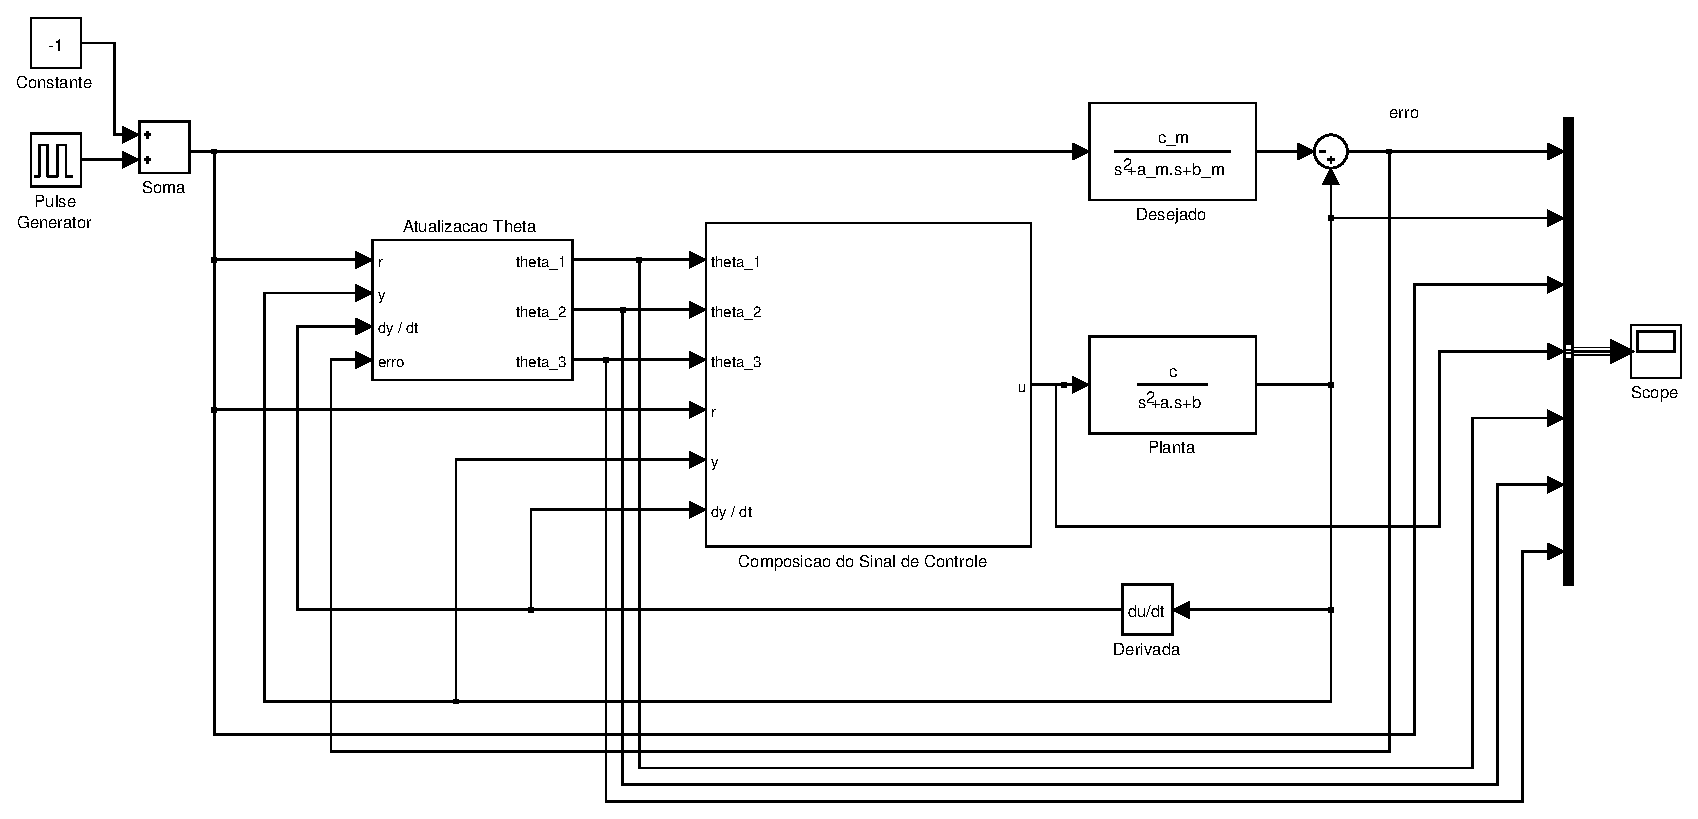
\includegraphics[width=0.95\textwidth]{imgs/questao3/sistema}
    \caption{Diagrama de blocos do sistema simulado.}
    \label{fig:q3_sistema}
\end{figure}

\begin{figure}[htb]
    \centering
    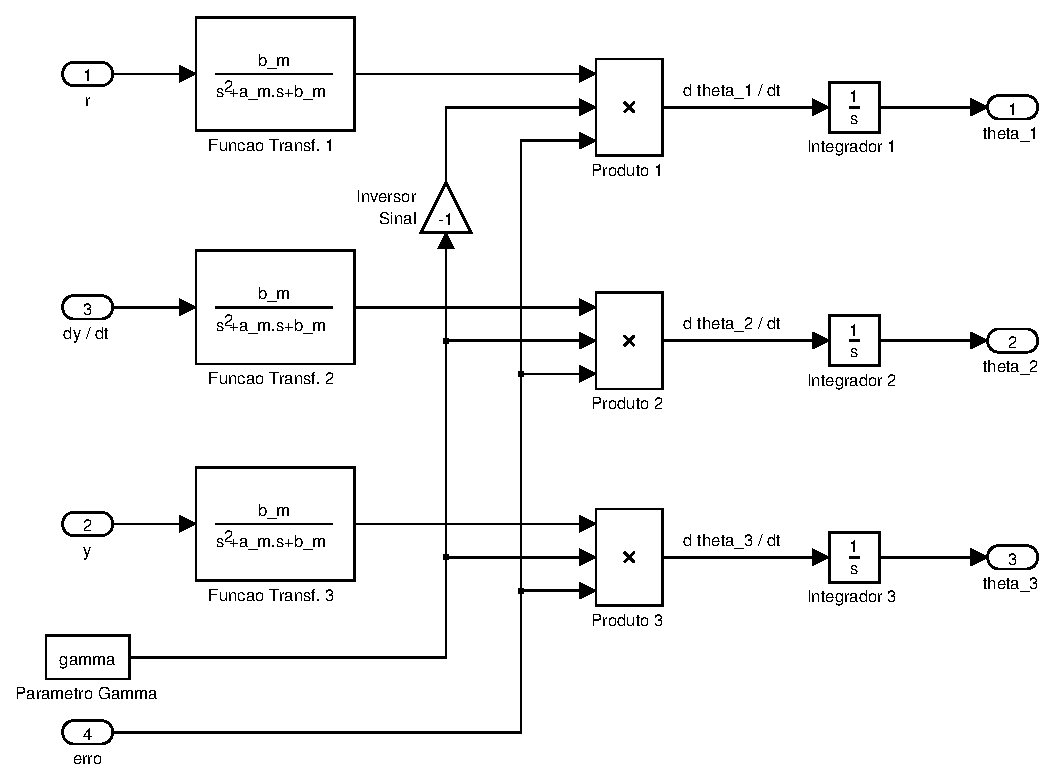
\includegraphics[width=0.8\textwidth]{imgs/questao3/theta}
    \caption{Diagrama de blocos do subsistema de atualização de $\theta$}
    \label{fig:q3_theta}
\end{figure}

\begin{figure}[htb]
    \centering
    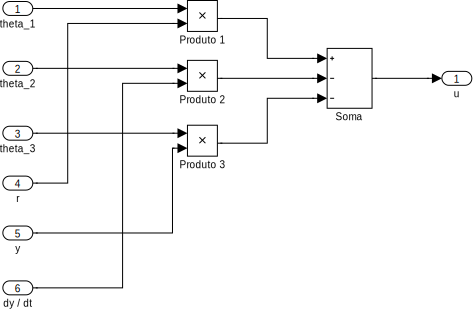
\includegraphics[width=0.6\textwidth]{imgs/questao3/sinal_controle}
    \caption{Diagrama de blocos do subsistema de composição do sinal de
             controle.}
    \label{fig:q3_sinal_cont}
\end{figure}

\begin{figure}[htb]
    \centering
    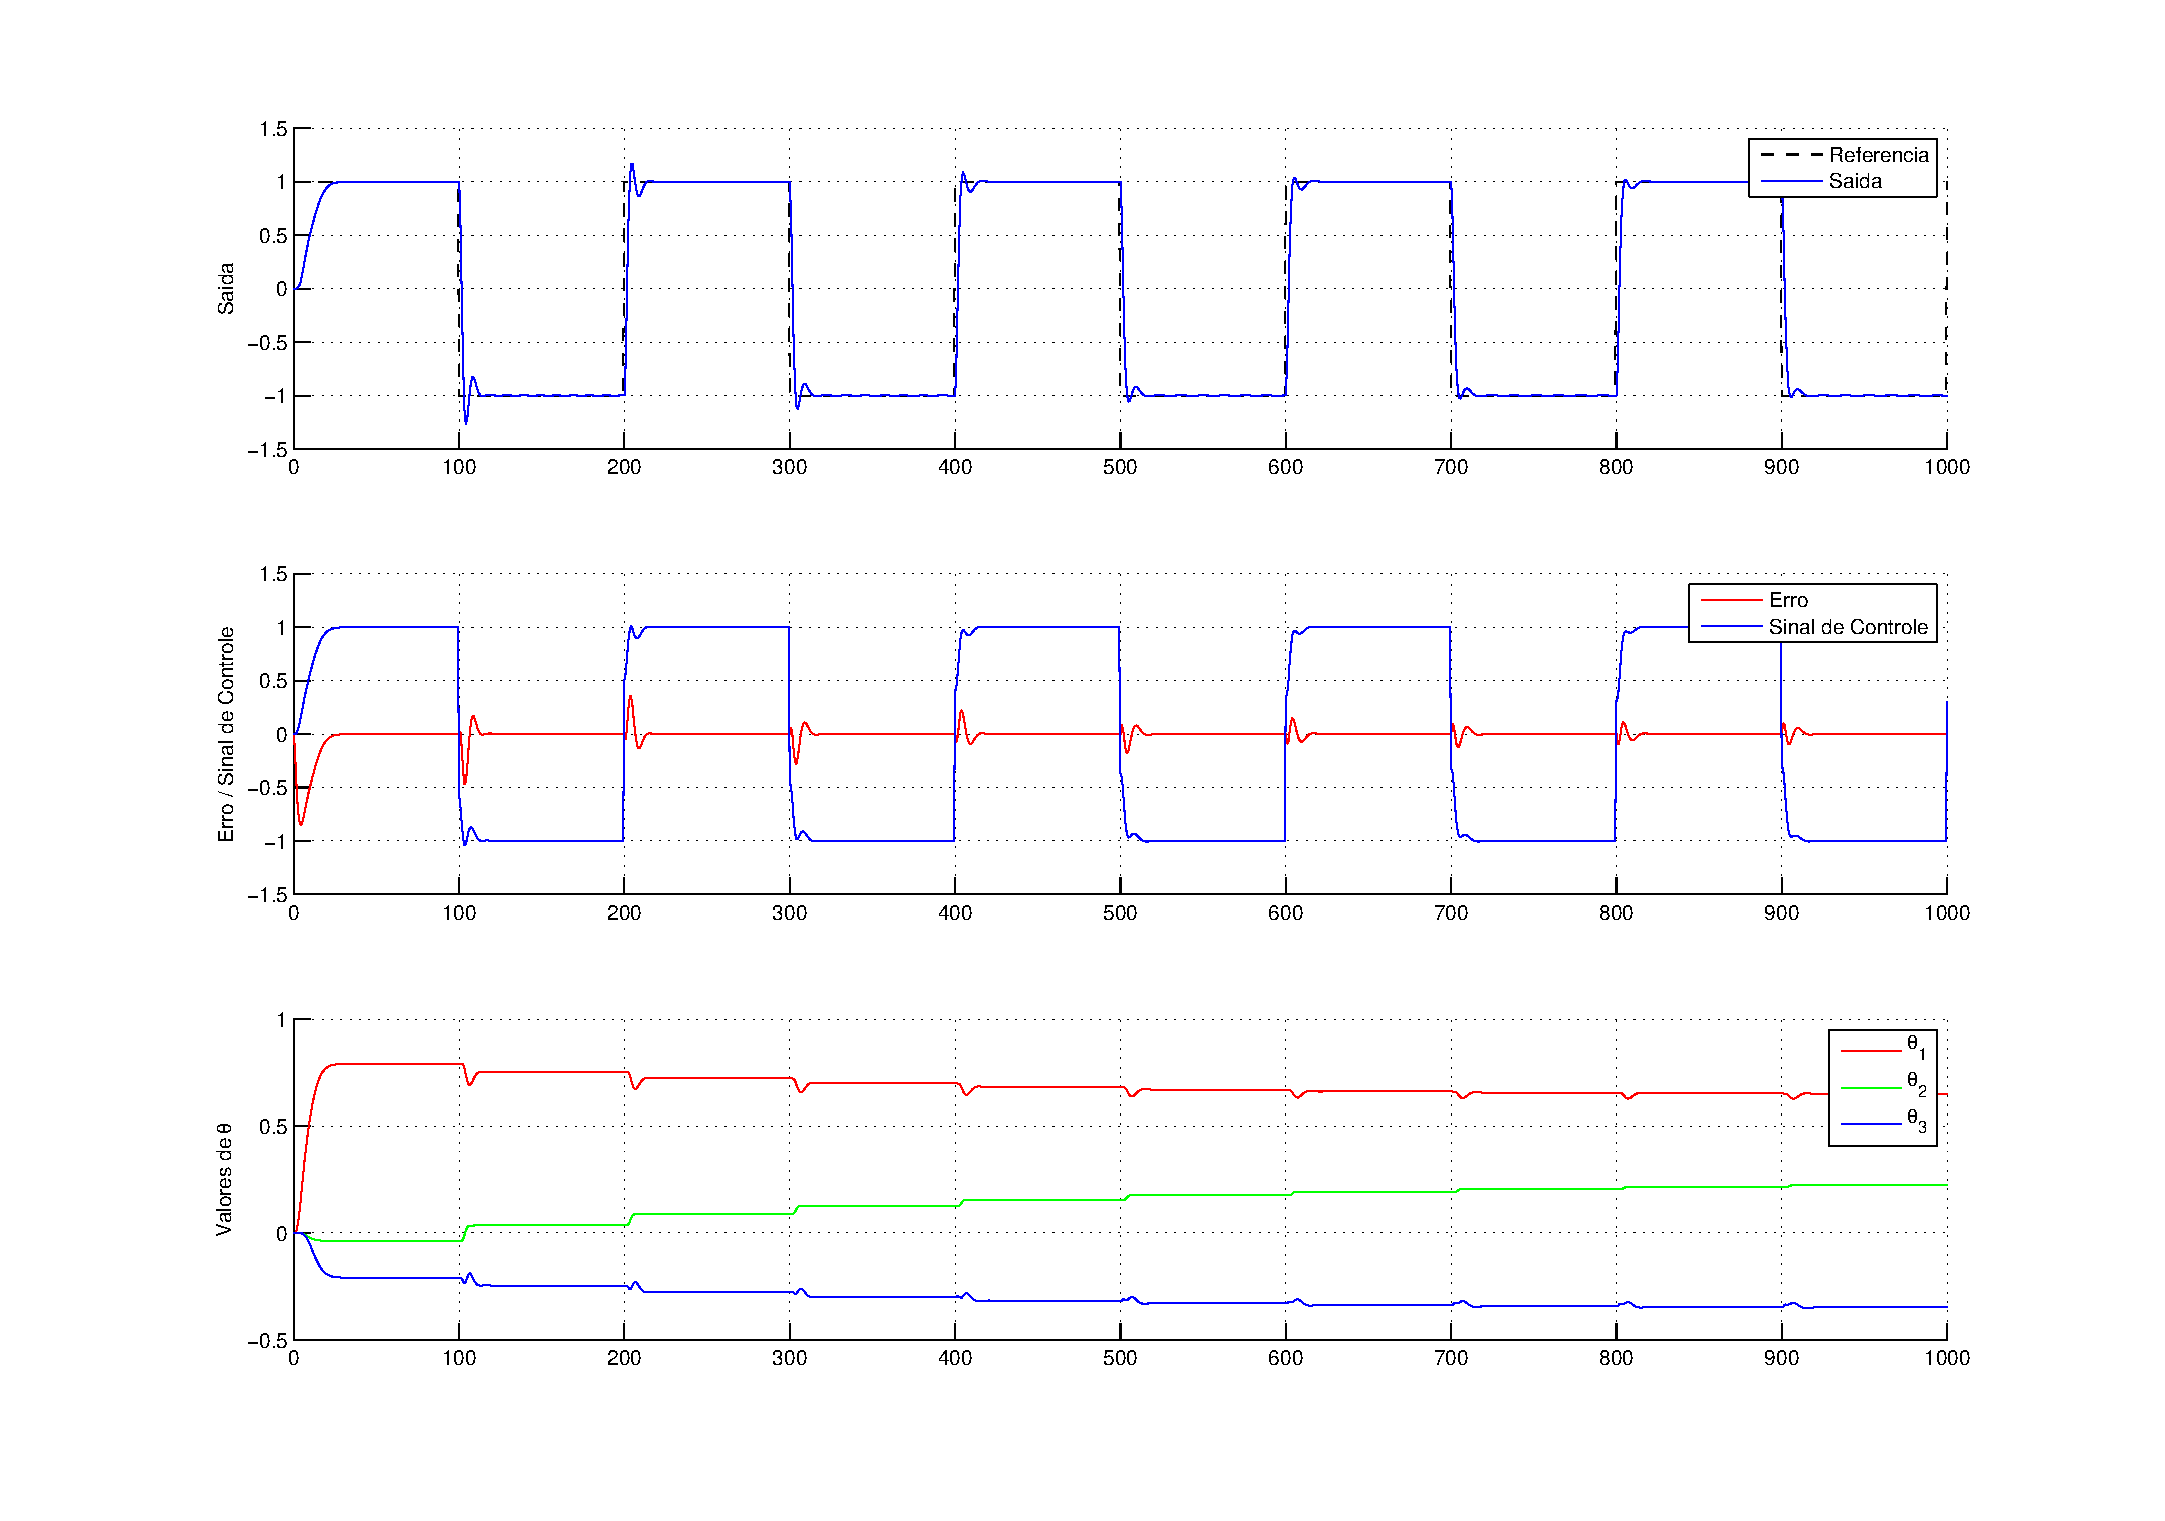
\includegraphics[width=0.95\textwidth]{imgs/questao3/saida_gamma_0.1.eps}
    \caption{Saída do sistema para $\gamma = 0.1$.}
    \label{fig:q3_saida_gamma_0.1}
\end{figure}

\begin{figure}[htb]
    \centering
    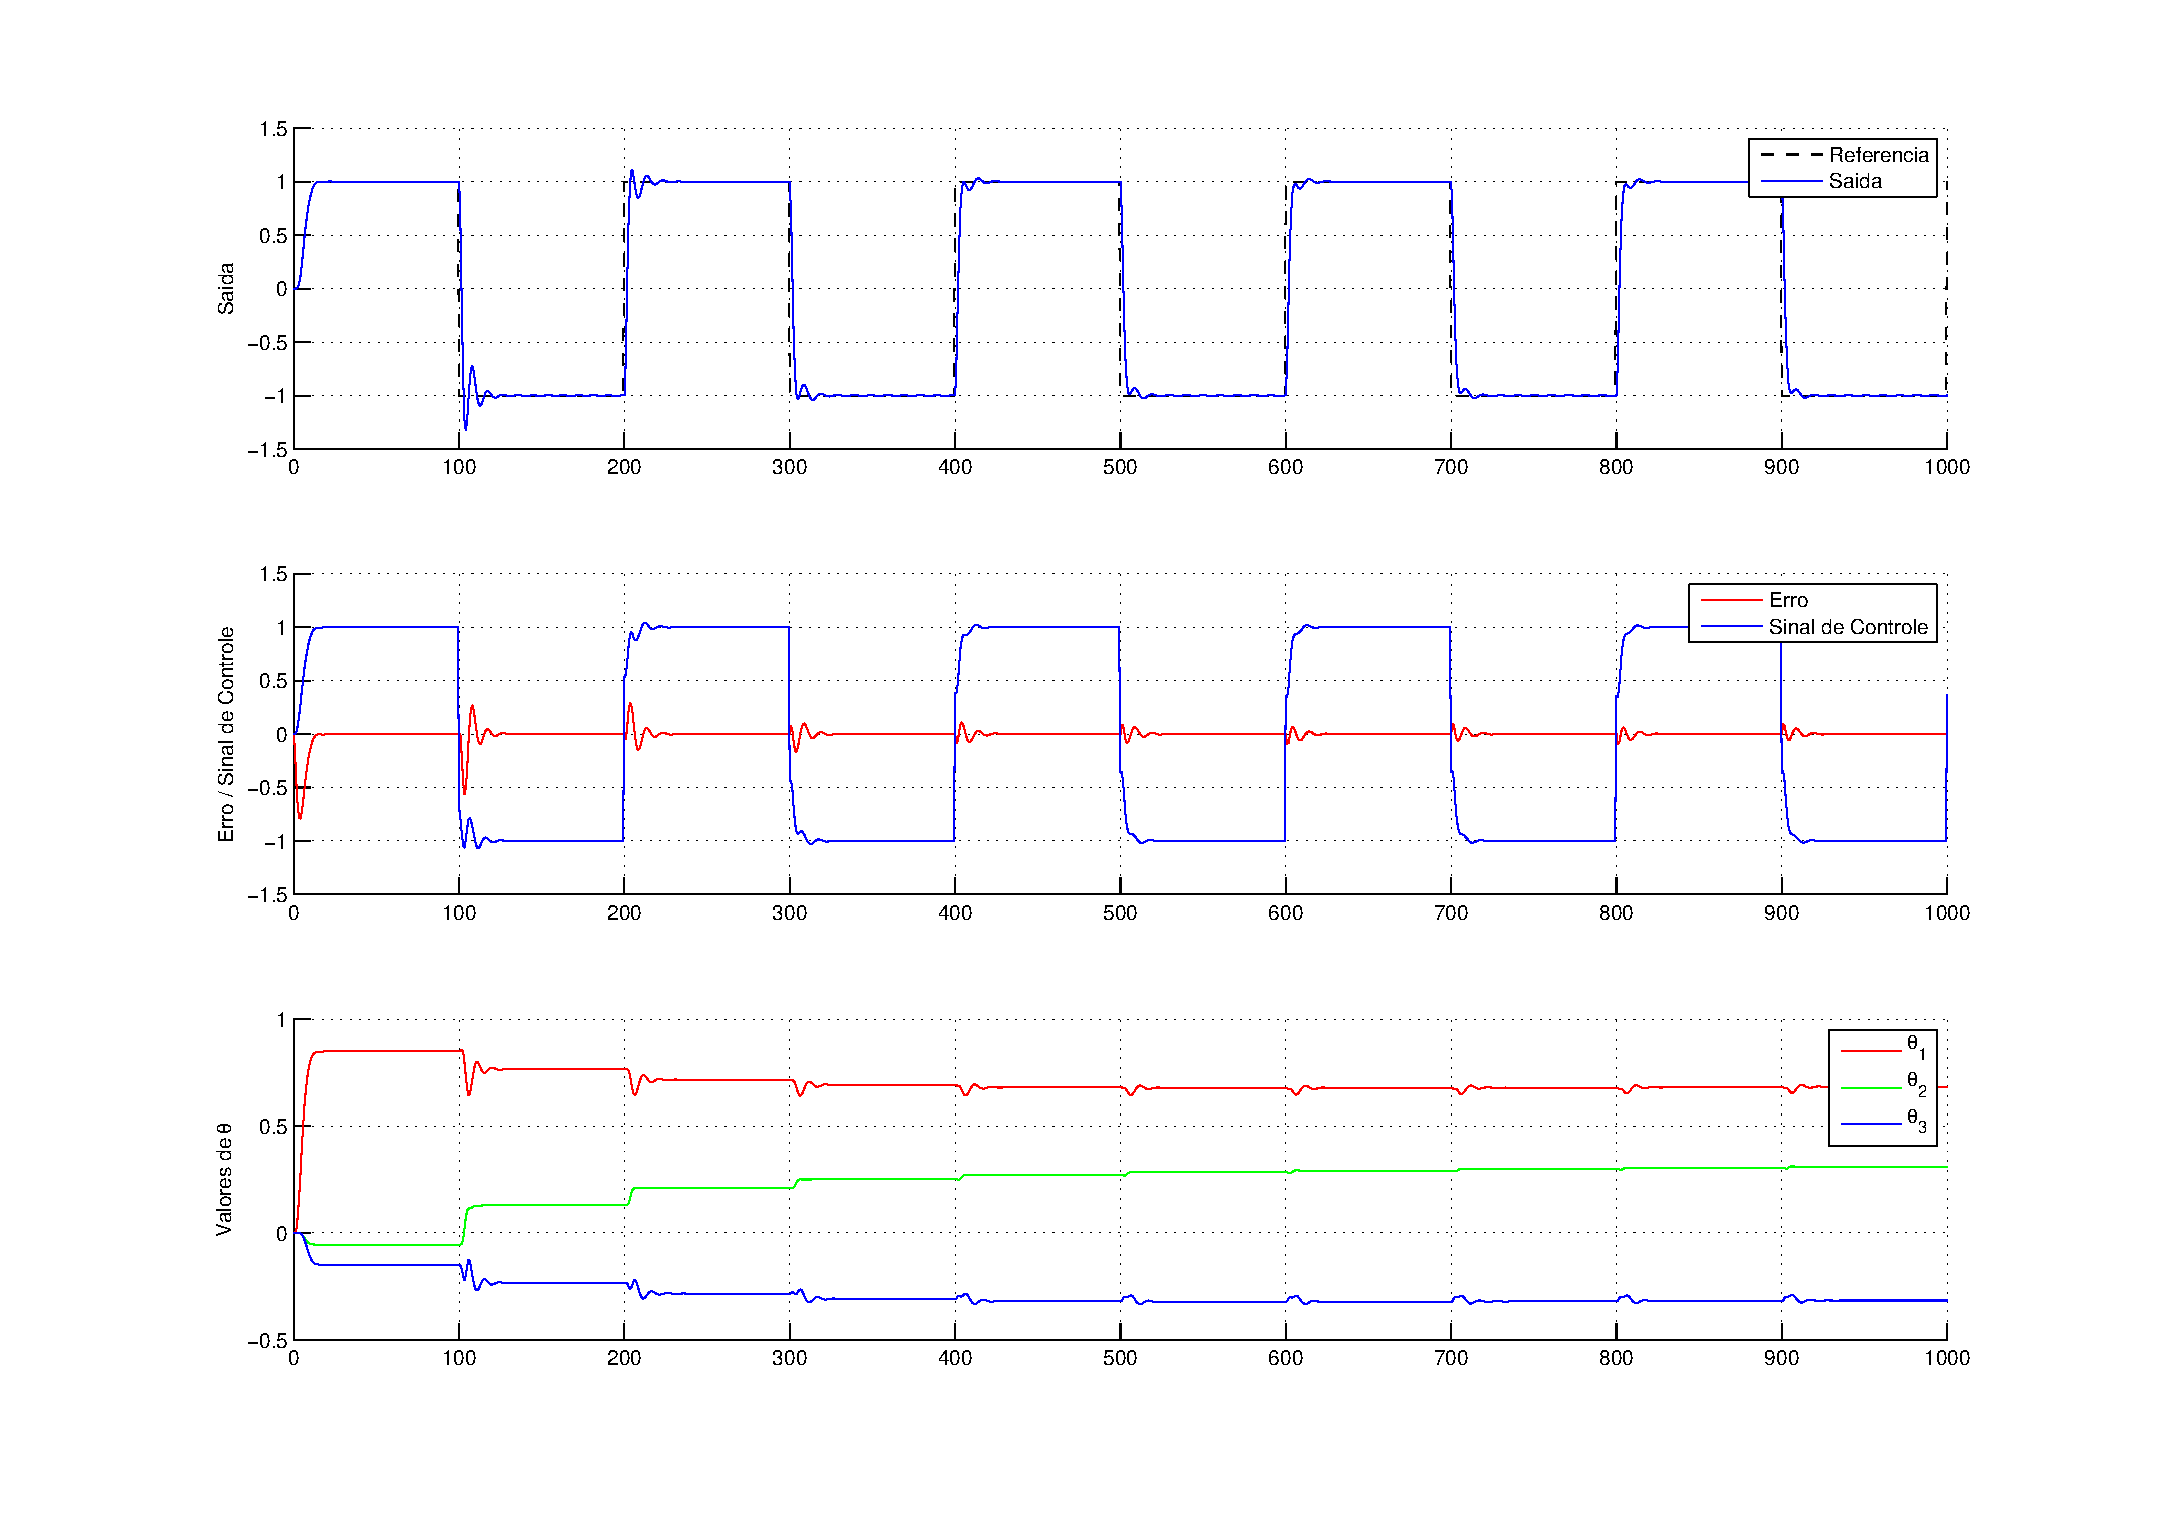
\includegraphics[width=0.95\textwidth]{imgs/questao3/saida_gamma_0.2.eps}
    \caption{Saída do sistema para $\gamma = 0.2$.}
    \label{fig:q3_saida_gamma_0.2}
\end{figure}

\begin{figure}[htb]
    \centering
    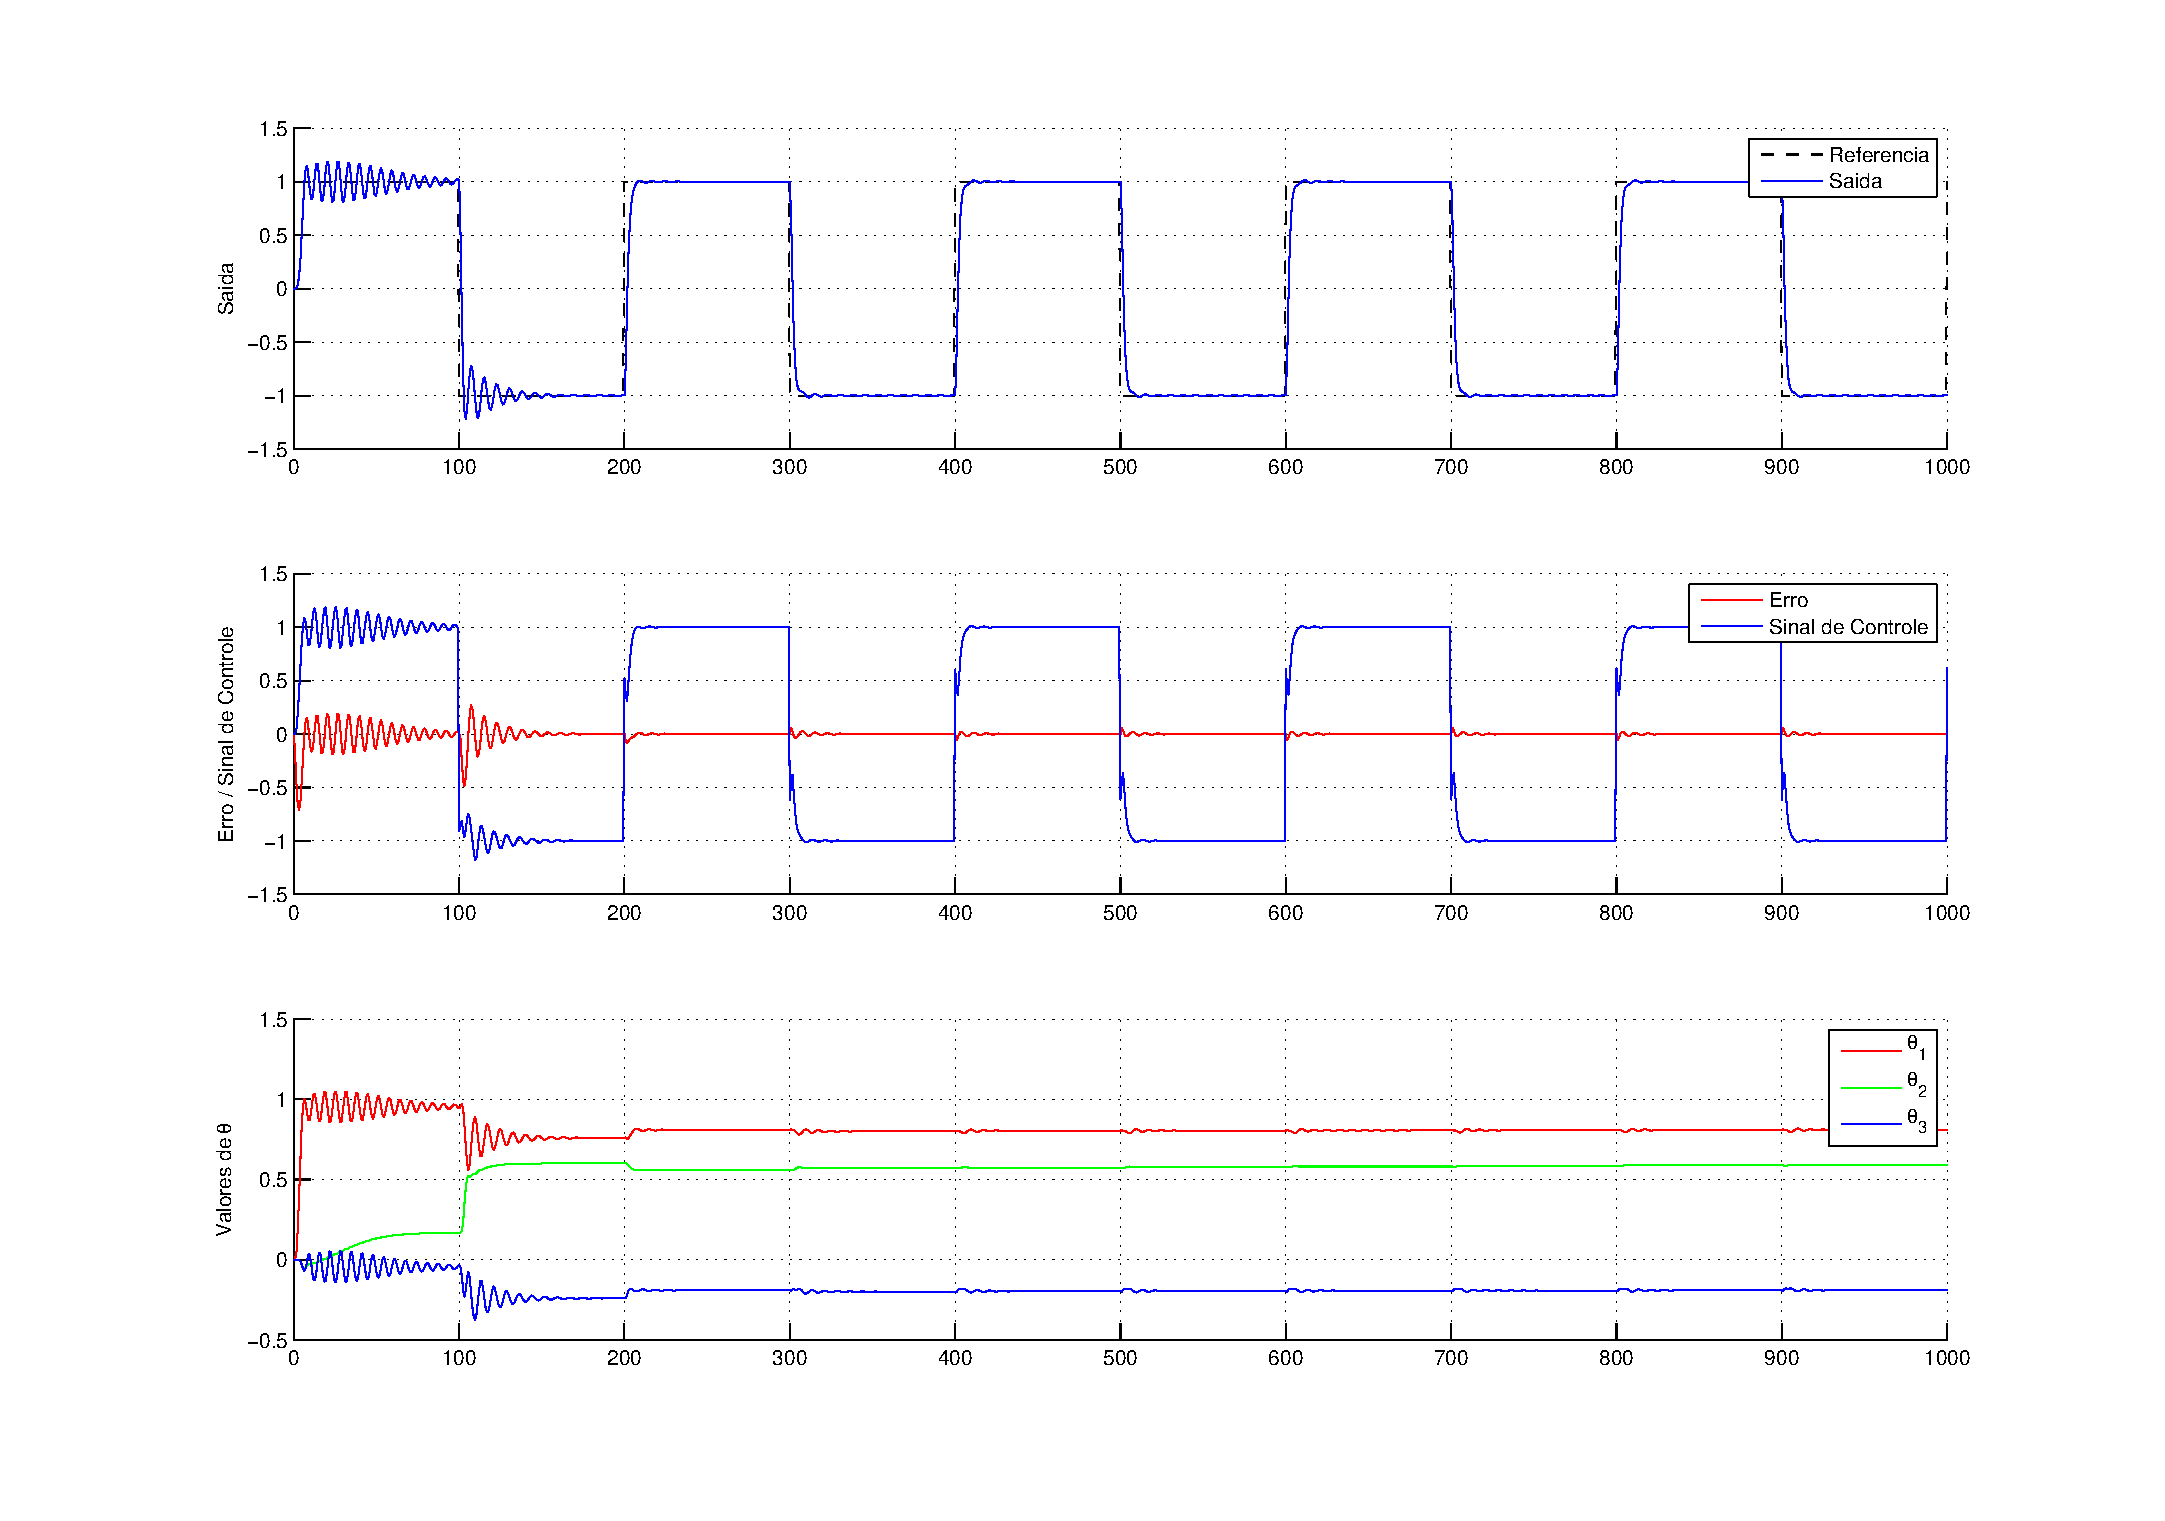
\includegraphics[width=0.95\textwidth]{imgs/questao3/saida_gamma_0.5.eps}
    \caption{Saída do sistema para $\gamma = 0.5$.}
    \label{fig:q3_saida_gamma_0.5}
\end{figure}

\begin{figure}[htb]
    \centering
    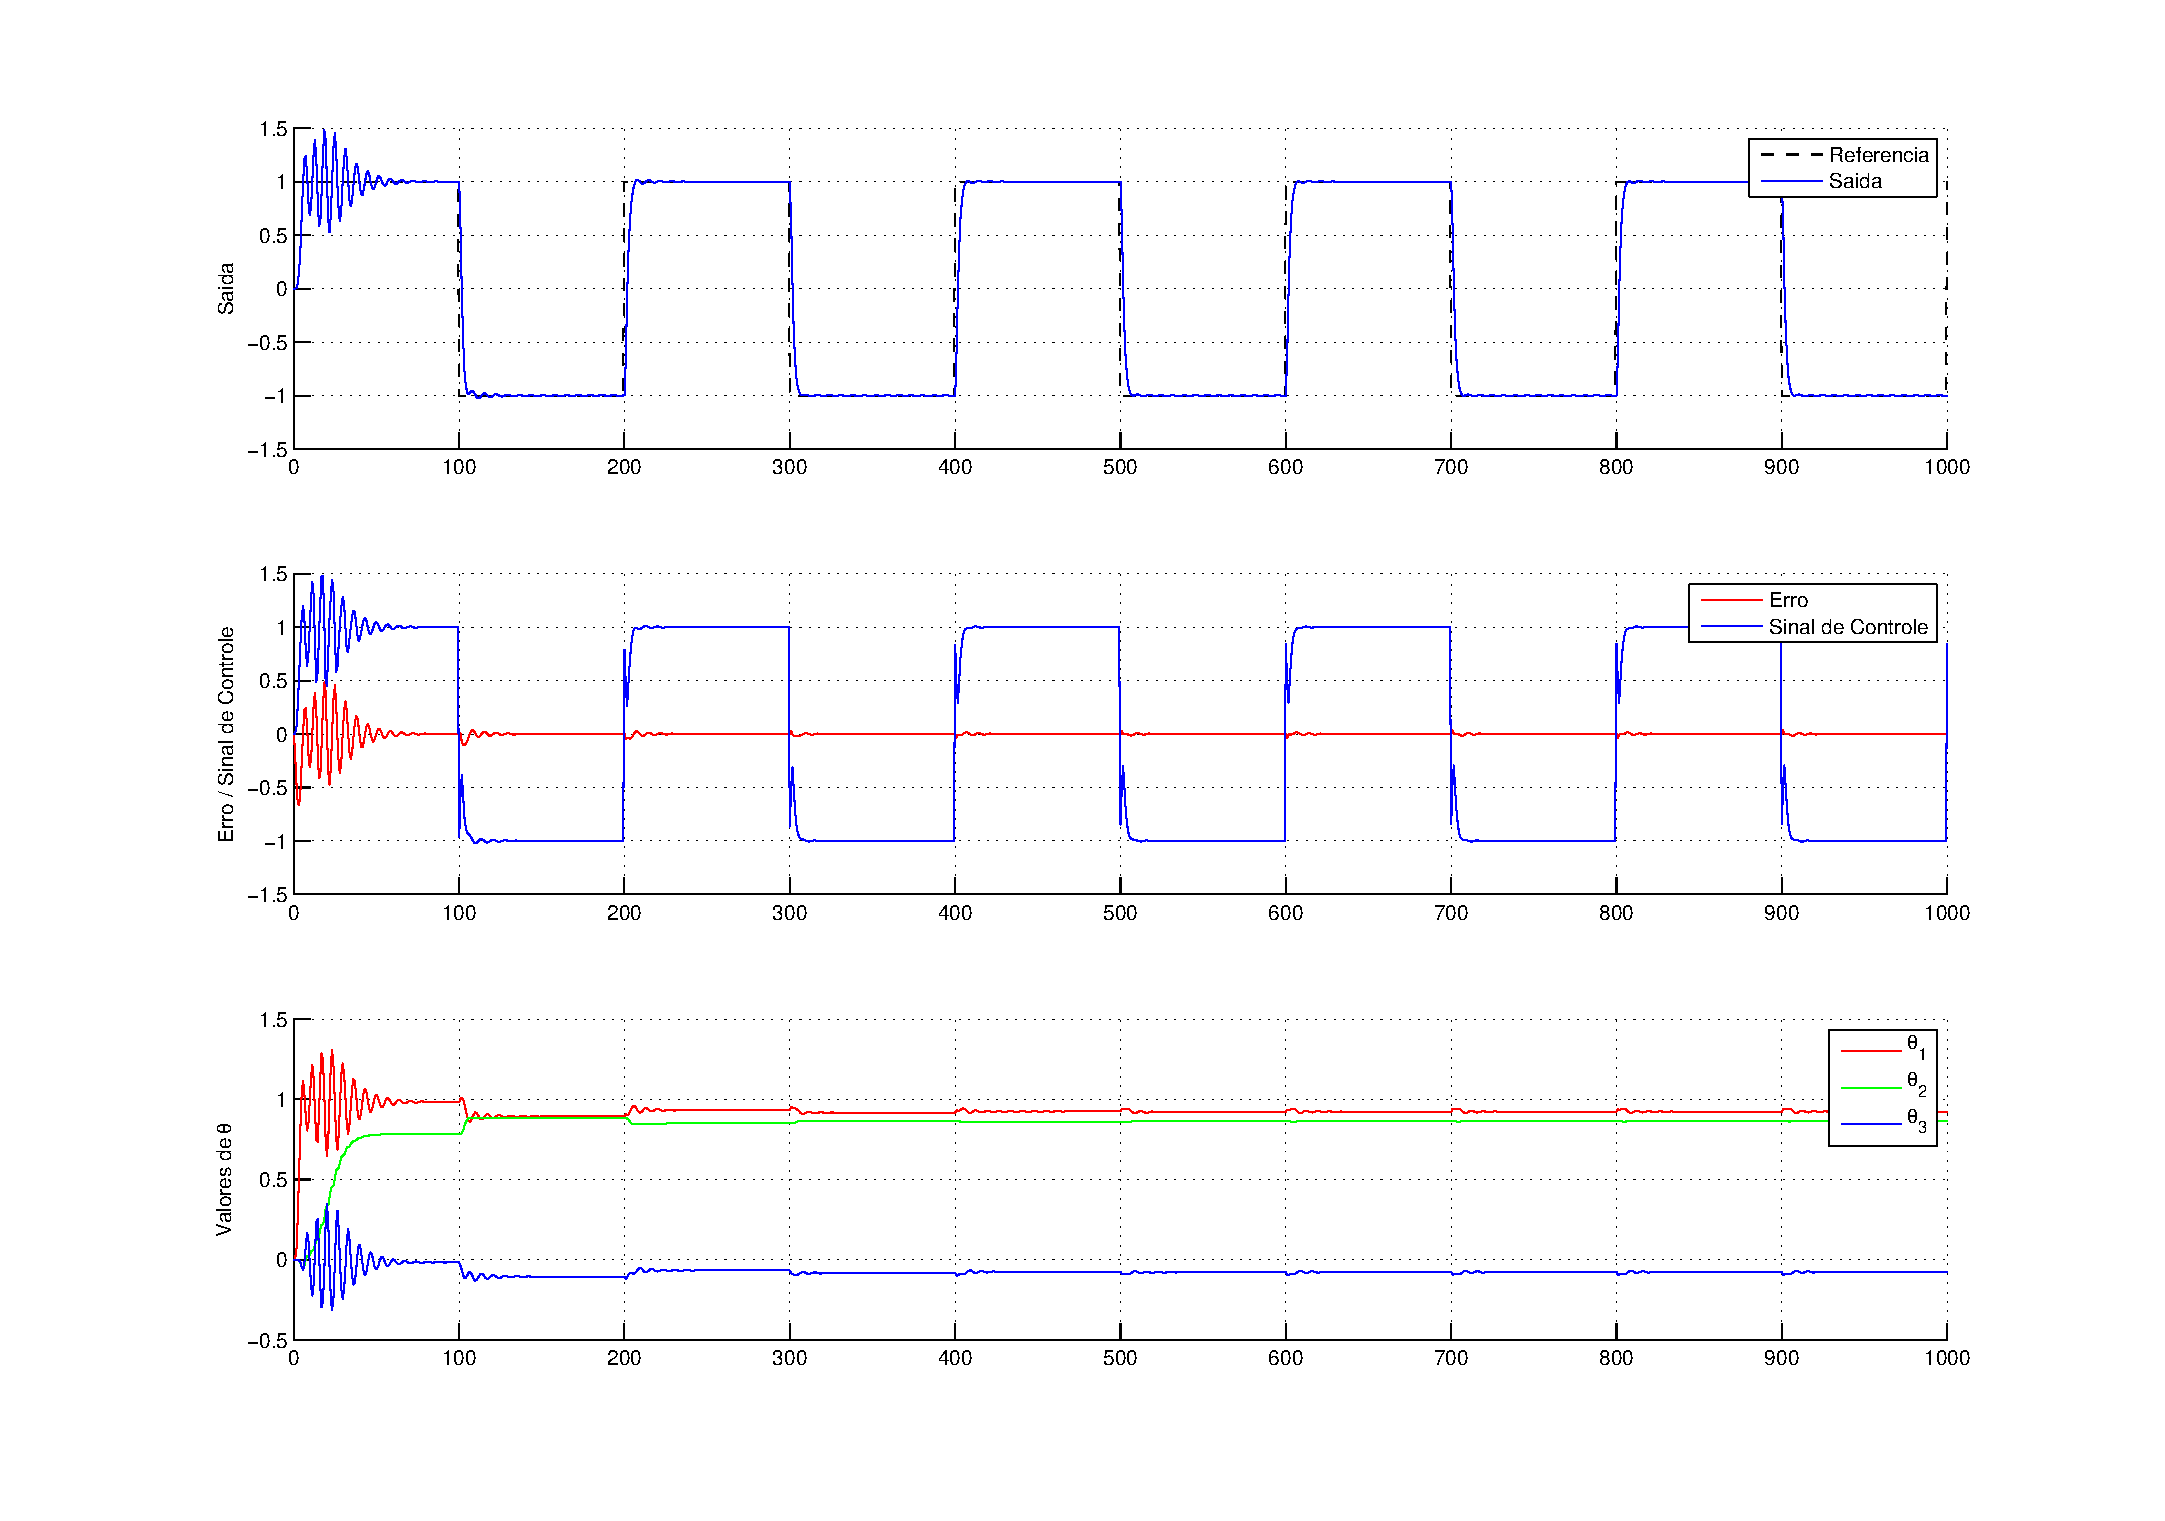
\includegraphics[width=0.95\textwidth]{imgs/questao3/saida_gamma_0.7.eps}
    \caption{Saída do sistema para $\gamma = 0.7$.}
    \label{fig:q3_saida_gamma_0.7}
\end{figure}

\begin{figure}[htb]
    \centering
    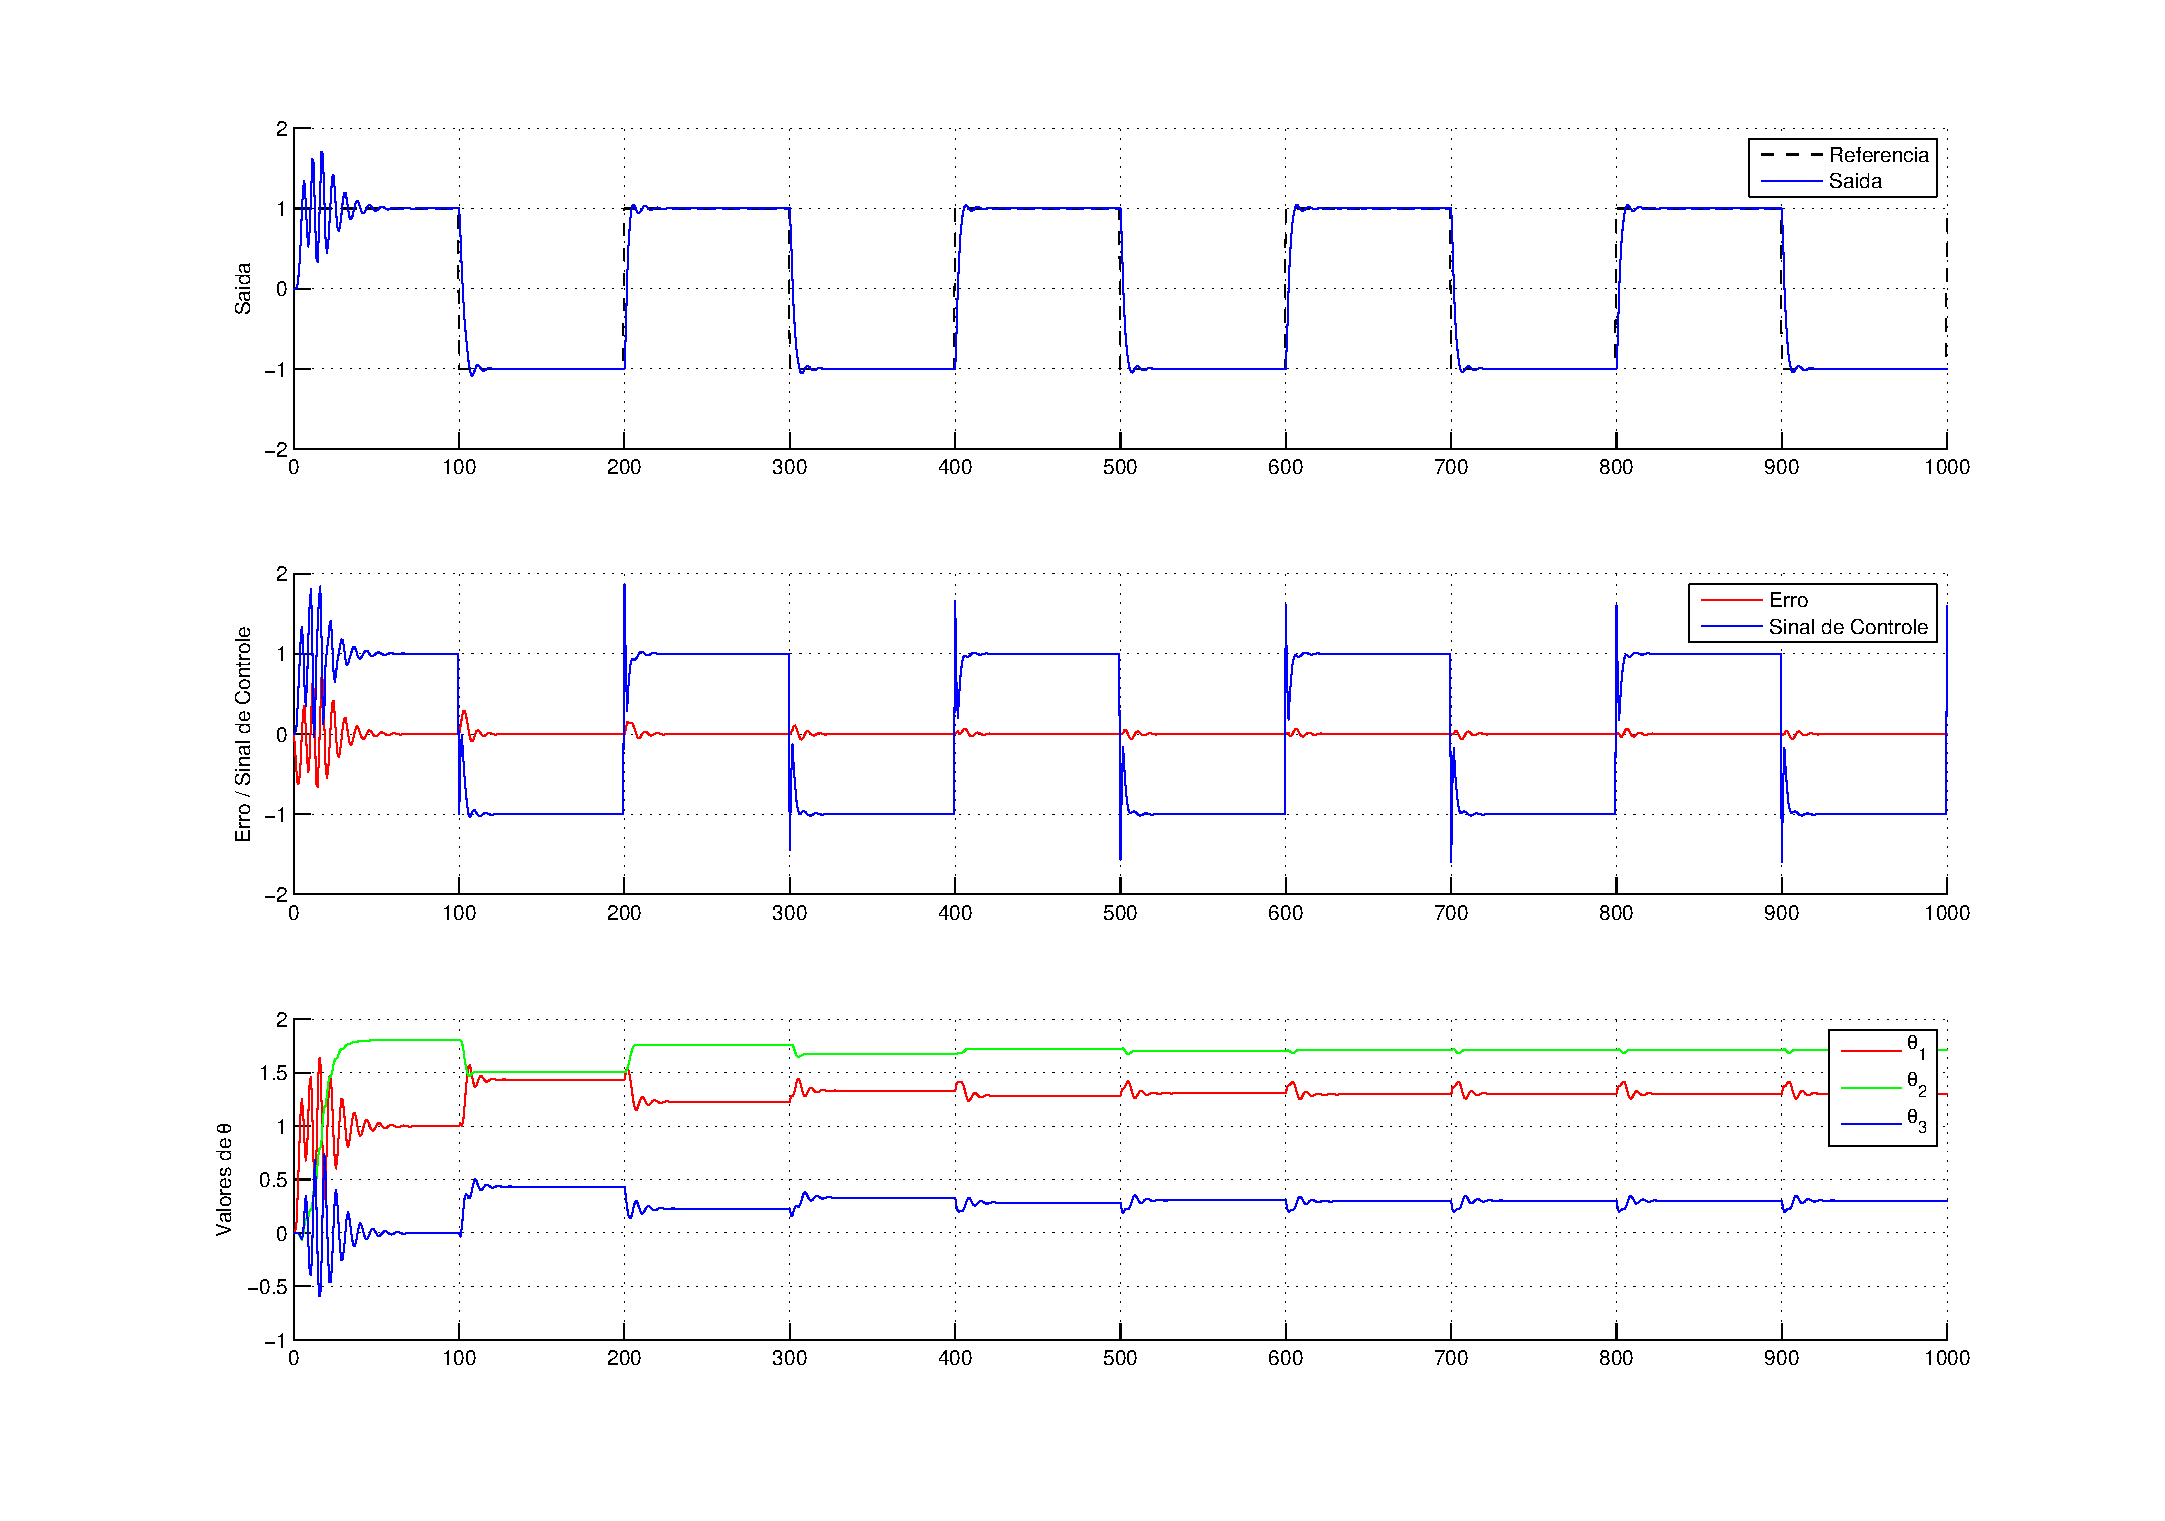
\includegraphics[width=0.95\textwidth]{imgs/questao3/saida_gamma_1.0.eps}
    \caption{Saída do sistema para $\gamma = 1.0$.}
    \label{fig:q3_sistema}
    \label{fig:q3_saida_gamma_1.0}
\end{figure}

O {\it script} do Matlab\textsuperscript{\textregistered} desenvolvido para a
resolução dessa questão pode ser encontrado no Apêndice \ref{ap:cod_q3}.
